\documentclass{aptpub}
%\documentclass{article}

\renewcommand{\baselinestretch}{1}
\usepackage{calc}
% \usepackage[paperwidth=\textwidth+2cm,paperheight=\textheight+2cm,%
% left=1cm,right=1cm,top=0.5cm,bottom=1.5cm]{geometry}

\usepackage[utf8]{inputenc}
\usepackage[american]{babel}
\usepackage{url}
\usepackage{amsmath,amsfonts}
\usepackage{subfigure}
\usepackage{tikz}
\usepackage{figlatex}
\usepackage[colorlinks=true]{hyperref}
\usepackage{arydshln}
\usepackage{multicol}
\definecolor{darkblue}{rgb}{0 0 .6}
\hypersetup{colorlinks=true,linkcolor=darkblue,citecolor=darkblue,urlcolor=darkblue}
\graphicspath{{../simu/}{}}
%\usepackage{amsthm}

\newcommand\expect[1]{\mathchoice{\bexpect{#1}}{\sexpect{#1}}{\sexpect{#1}}{\sexpect{#1}}}
\newcommand\bexpect[1]{\mathbb{E}\left[#1\right]}
\newcommand\sexpect[1]{\mathbb{E}[#1]}
\newcommand\variance[1]{\mathrm{var}\left[#1\right]}
\newcommand\svariance[1]{\mathrm{var}[#1]}
\newcommand\proba[1]{\mathchoice{\bproba{#1}}{\sproba{#1}}{\sproba{#1}}{\sproba{#1}}}
\newcommand\bproba[1]{\mathbb{P}\left(#1\right)}
\newcommand\sproba[1]{\mathbb{P}(#1)}
\newcommand\Sp{\mathcal{S}} %% state space
\newcommand\F{\mathcal{F}} %% state space
%\newcommand\N{\mathbb{Z}^+}
\newcommand\R{\mathbb{R}}
\newcommand\Z{\mathbb{Z}}
\newcommand\bX{\mathbf{X}}
\newcommand\bY{\mathbf{Y}}
\newcommand\bZ{\mathbf{Z}}
\newcommand\ceil[1]{\lceil#1\rceil}
\newcommand\floor[1]{\lfloor#1\rfloor}
\newcommand\abs[1]{\mathchoice{\babs{#1}}{\sabs{#1}}{\sabs{#1}}{\sabs{#1}}}
\newcommand\babs[1]{\left|#1\right|}
\newcommand\sabs[1]{|#1|}
\newcommand\norm[1]{\mathchoice{\bnorm{#1}}{\snorm{#1}}{\snorm{#1}}{\snorm{#1}}}
\newcommand\bnorm[1]{\left\|#1\right\|}
\newcommand\snorm[1]{\|#1\|}
\newcommand\lp{\left(}
\newcommand\rp{\right)}
\newcommand\p[1]{\left(#1\right)}
\newcommand\parray[1]{\left(\begin{array}{c}#1\end{array}\right)}
%\newcommand{\bydef}{\stackrel{\rm{def}}{=}}
\newcommand{\bydef}{:=}
\newcommand{\toprob}{\stackrel{\mathcal{P}.}{\rightarrow}}
\newcommand\red[1]{{\color{red}#1}}

\newcommand\numax{\nu_{\max{}}}
\newcommand\numin{\nu_{\min{}}}



%%%%%%%%%%%%%%%%%%%%%%%%%%%%%%%%%%%%%%%%%%
\authornames{N. Gast and B. Gaujal}
\shorttitle{Computing Absorbing Times via Fluid Approximations}


\begin{document}





%%%%%%%%%%%%%%%%%%%%%%%%%%%%%%%%%%%%%%%%%%%%%%%
\title{Computing Absorbing Times via Fluid Approximations}

\authorone[Inria]{Nicolas Gast}

\addressone{University of Grenoble Alpes and Inria, Grenoble, France}

\authortwo[Inria]{Bruno Gaujal}

\addresstwo{University of Grenoble Alpes and Inria, Grenoble, France}





\begin{abstract}

  In this paper, we compute the absorbing time $T_n$ of a
  $n$-dimensional discrete time Markov chain made of $n$ components,
  each with an absorbing state and evolving in mutual exclusion. We
  show that the random absorbing time $T_n$ is well approximated by a
  deterministic time $t_n$ that is the first time when a fluid
  approximation of the chain approaches the absorbing state at a
  distance $1/n$.  We provide an asymptotic expansion of $t_n$ that
  uses the spectral decomposition of the kernel of the chain as well
  as the asymptotic distribution of $T_n$, relying on extreme values
  theory.  We show the applicability of this approach with three
  different problems: the coupon collector, the erasure channel
  lifetime and the coupling times of random walks in high dimensional
  spaces.
\end{abstract}



\keywords{Markov chain, Fluid approximation, Extreme values, Coupon collector, Coupling time}


\ams{05D40}{60J10;37A25}

\section{Introduction.}


Analyzing stochastic discrete event dynamic systems by constructing
deterministic fluid approximations (sometimes called hydrodynamic
limits) has been very popular in recent years.  This technique is very
powerful to get fast and accurate performance evaluation of computer
based systems
\cite{Leboudec2,chaintreau2009age,gast2010mean}.  It can
be applied quite generally to study the transient behavior or the
convergence to stationary or quasi-stationary distributions
\cite{Leboudec,Ramanan,Meleard}. 




In this paper, we rather consider the case where we want to
approximate a finite (but large) stochastic system over a {\it
  stopping time} of the process.
We consider a Markov chain $\bX:=(X_1\dots X_n)$, where $X_i$ is
called the $i$th component. The components are all Markov chains that
have an absorbing state (say state $0$) and respective transition
matrices $P_1, \ldots, P_n$.  The evolution of $\bX$ is as follows: At step
$t$, a single component is chosen according to a fixed probability
vector $(p_1,\ldots, p_n)$ and the chosen component (say $i$) makes
one transition, according to its kernel $P_i$.  Our goal is to compute
the first instant $T_n$ when all components have reached their
absorbing state.



The simplest example of such a system is the coupon collector. Each
coupon is seen as a Markov chain with two states. The absorbing state
($0$) corresponds to the presence of the coupon in the current
collection and the other state ($1$) to its absence:
\begin{center}
  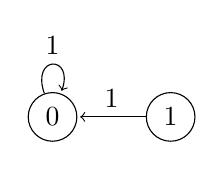
\begin{tikzpicture}[shorten >=1pt,xscale=1.5]
    \node[circle,draw] at (0,0) (0) {0};
    \node[circle,draw] at (1,0) (1) {1};
    \draw (1) edge[->] node[above] {1} (0);
    \draw (0) edge[->,loop above] node[above] {1} (0);
  \end{tikzpicture}
\end{center}
In the original coupon collect, all the chains $X_1\ldots X_n$ have
this transition matrix and the choice probability vector is uniform:
$p_i=1/n$ for $i\in\{1\dots n\}$.




The coupon collector, or one of its generalizations, appears naturally
in the analysis of distributed algorithms, for example in
\cite{flajolet1992birthday,ganesh2010load}.  Given its importance,
several generalizations of the coupon collector have been studied in
the literature. Many of them fall in our general model.  In
\cite{neal2008generalised}, the author studies the asymptotic
distribution of the tail-distribution of the time to collect a
collection under a non-uniform \emph{i.i.d.} distribution of coupons.
In \cite{doumas2012coupon}, the authors study a non-uniform coupon
(coupons are \emph{i.i.d.} with non-uniform probabilities) and obtain
the asymptotic behavior of the variance of the time to collect $n$
coupons.  
In \cite{anceaume2015} the authors study the time to collect $c<n$
different coupons. They show that the uniform coupon is often a
best-case scenario for the hitting time in many cases.  Our model of
heterogeneous coupon is close to the one of
\cite{doumas2014coupon,doumas2012coupon} that studies asymptotic
properties of the problem of collecting $n$ different coupons, where
coupon $i$ has probability $p_i=a_i/\sum_{j=1}^n a_j$. They fix a
sequence $a_i$ and study asymptotic properties.
Our problem can also be seen as a special case of the coupon collector with
random quotas studied in \cite{may2008coupon,shank2013coupon} where
the authors study the time to collect $m_i$ coupons of type $i$, where
$m_i$ is a random variable. Our paper differs on two points: (i) from
a modeling point of view, we focus on the case where $m_i$ is the
hitting time of a Markov chain, and (ii) the authors use generating
functions while we use a fluid approximation. With our model, we are able to use extreme value theory to obtain close-form
expression for asymptotic distribution and moments. 


\paragraph*{Contributions}
In this paper, we compute an asymptotic equivalent $t_n$ of the
absorbing time $T_n$
under weak assumptions on $p_n$ (see Section~\ref{sec:homo} for a
precise statement).  The approximation $t_n$ is obtained by defining a
fluid approximation of ${\bf X}:=(X_1\dots X_n)$ and by computing the
time when this fluid approximation is at a distance $1/n$ from the
absorbing state.  Our main result is to show that $T_n$ is asymptotic
equal (in distribution) to $t_n$ plus a Gumbel distribution with mode
$0$ and scale $1/\nu\min_ip_i$, plus a negligible sub-linear term
$o(n)$. The exponent $\nu$ depends on the eigenvalues of the
transition matrices.  We also provide closed forms expressions for the
asymptotic expectation of $T_n$ and its moments.

The deterministic time $t_n$ is easier to compute that its stochastic
counterpart $T_n$.  When all chains have the same transition matrix and
$p_i=1/n$, we show that
$t_n=(1/\nu) n\log n + ((d-1)/\nu)n\log\log n + O(n) $, where $-\nu$
is the eigenvalue of $Q$ with the largest real part (which is a real
negative number) and $d$ depends on its multiplicity.  We apply this
to the coupon collector in which case $-\nu=1$ (see
Section~\ref{sec:cc}) as well as to random walks in finite grids (see
Section~\ref{sec:rw} where we give an equivalent to the coupling time
in grids with or without drifts).  We also provide bounds on $t_n$
based on the absorbing time of a single component in
Section~\ref{sec:erasure}.  In the heterogeneous and/or non-uniform
cases, $t_n$ can often only be computed numerically (see
Section~\ref{sec:non_unif} for a numerical application to the coupon
collector with rare coupons).

Our proofs rely on two ingredients. First, we use a classical
``Poissonization technique'' to transform the system of $n$ coupled
Markov chains into a continuous time Markov chain made of $n$
independent components.  Second, we use ideas from extreme value
theory to relate $T_n$ and the time when the fluid approximation
approaches $1/n$.


\paragraph*{Road-map} The rest of the paper is organized as follows.
We introduce the model and the definition of $t_n$ in
Section~\ref{sec:problem}. We develop the equivalence theorems between
$t_n$ and $T_n$ is Section~\ref{sec:results}. We present the
applications to the coupon collector in Section~\ref{sec:cc}, where we
also show how to compute a bound
(Theorem~\ref{th:absorbing_bound}). Next, we show how this can be applied to
compute the coupling time of random walks in
Section~\ref{sec:rw}. Finally, we conclude in
Section~\ref{sec:conclusion}.

\section{Problem statement.}
\label{sec:problem}

We consider a discrete-time finite Markov chain $\bf X$ made of $n$
chains: $X_1,\ldots, X_n$. The chain $X_i$ called component~$i$ in the
following. All components have an absorbing state $0$ and respective
transition matrices $P_1, \ldots, P_n$.  The component $X_i$ lives in
a finite state space $\{0\dots k\}$ and $0$ is an absorbing state:
$P_i(0,0)=1$.  We assume that the state $0$ is reachable from any
initial state, which implies that with probability one, each component
hits $0$ in finite time.  For reasons that will become clear in the
next section, the transition matrix $P_i$ will be decomposed as
\begin{equation}
  P_i = \left[
    \begin{array}{cc}
      1&\mathbf{0}\\
      \mathbf{q}_i & I+Q_i
    \end{array}
  \right],
\label{eq:defQ}
\end{equation}
where $Q_i$ is a $k\times k$ rate matrix with the following
properties: $Q_i$ is non-singular, for all $a$, $\sum_{b}Q_i(a,b)\le0$
and there exists at least one state $a$ such that
$\sum_{b} Q_i(a,b) < 0$.

Let $p=(p_1\geq \dots \geq p_n)$ a probability distribution on
$\{1\dots n\}$. The discrete-time Markov chain $\bX=(X_1\dots X_n)$ is
defined by the following dynamics. At time $0$, each $X_i(0)$ is
picked independently according to an initial distribution $\alpha_i$
($(\alpha_i)_0 = 0$, because  component~$i$ is not in its  absorbing state initially, so that we denote by $\alpha_i$ the $k$-dimensional row vector
$((\alpha_i)_1\dots (\alpha_i)_k$).  Then at each time step $t$, one
coordinate $i$ is picked with probability $p_i$, independently of the
past. Then, the $i$th coordinate, $X_i$, makes one transition
according to the matrix $P_i$.

In what follows, we characterize $T_n$, the hitting time of
$(0,0,\dots,0)$:
\begin{align*}
  T_n:=\inf \{t \text{ such that }\forall i\in\{1\dots n\}:
        X_i(t)=0\}
\end{align*}


We distinguish several cases in the analysis of this problem.  We say
that the chain is {\it homogeneous} if all components $X_1\dots X_n$
have the same transition matrix $P$, and the same initial distribution
$\alpha$.  From this point on, we assume homogeneity, unless it is
specified otherwise.  The non-homogeneous case is treated in
Section~\ref{sec:hetero}.  We say that $\bf X$ is {\it uniform} if the
choice probabilities among the components are all equal:
$(p_1,\dots,p_n) = (1/n,\ldots, 1/n)$.
In the following, we will show that when $n$ is large, $T_n$ is well
approximated by a deterministic time $t_n$ that we define below. 


\subsection{Definition of $t_n$ in the uniform and homogeneous case.}
\label{ssec:defhomo}

In the uniform and homogeneous case, we define $t_n$ to be the unique
solution of the following equation, using $Q = Q_i$ for all $i$, as
defined in \eqref{eq:defQ}, $\alpha$, the initial distribution vector of
each component and $\mathbf{1}$, the $k$-dimensional column vector whose elements are all equal to 1.
\begin{equation}
  \frac{1}{n} = \alpha\exp(Qt_n/n)\mathbf{1},
  \label{eq:deftn}
\end{equation}
where $\mathbf{1}$ denotes the $k$-dimensional column vector whose
elements are all equal to $1$.

This definition is justified by using a dynamical system that is a
mean field limit of the Markov chain.  We define the empirical
measure, $(M_0,M_1,\dots ,M_k)$ of the chain:
\begin{equation*}
  M_a(t) \bydef \frac{1}{n} \sum_{i=1}^n {\delta}_{\{X_i(t) = a\}}.
\end{equation*}
By the definition of $Q$ given in \eqref{eq:defQ}, for all
$a \not= 0$, we have
\begin{align*}
  \expect{M_a(t+1) - M_a(t)|{\bf M}(t)} 
  & =  \frac1n\sum_{b} M_b(t) Q(b,a).
\end{align*}
When the number of components becomes large, the empirical measure
$(M_0,M_1,\dots ,M_k)$ converges to a deterministic population
$(m_0,m_1,\dots ,m_k)$ whose dynamics is given by an ordinary
differential equation (ODE) (see \cite{Kurtz} for example).  In matrix
form, and focusing on the $k$-dimensional vector
${\bf m} \bydef (m_1,\dots ,m_k)$ (removing the coordinate $m_0$),
this equation can be written
\begin{align}
 \dot{\bf m}(t) =  \frac{1}{n} {\bf m}(t) Q.
\label{eq:ode}
\end{align}

This ODE is linear and its solution can be computed explicitly.  The
sum $m(t) \bydef \bf m \cdot \mathbf{1}$ is equal to
$m(t)=\alpha\exp(Qt/n)\mathbf{1}$.

When $n$ is large, the proportion of components not yet in state $0$
can be approximated by $m(t)$. % :

Notice that,  unlike in the finite case,   $m(t)$ never reaches $0$.  
However,  since in  the system with $n$ components  $M_1(t)+ M_2(t) + \cdots + M_k(t)$ reaches $0$ as soon as it becomes smaller than $1/n$, 
a 
good fluid approximation of the stopping time $T_n$ should be obtained by setting
\begin{equation}
  t_n := \inf\{t>0 \text{ such that } m(t)=\frac1n\}.
\end{equation}
This  definition implies that  $t_n$ is the solution of Equation
\eqref{eq:deftn}.


\subsection{Definition of $t_n$ in the non-uniform or non-homogeneous
  case.}
\label{ssec:defhetero}

Let us now consider the non-homogeneous, non-uniform case, with a
general choice vector $(p_1,\dots,p_n)$.  We always assume with no
loss of generality that $p_1 \geq p_2\geq \cdots \geq p_n$.  We do not
construct explicitly the population dynamics but jump directly to the
analog of Equation \eqref{eq:deftn}.

If one considers the evolution of the $i$th chain, independently of
the rest, it is a Markov chain with transition matrix
\begin{equation*}
  \left[
    \begin{array}{cc}
      1&\mathbf{0}\\
      p_i \mathbf{q}_i & I+ p_i Q_i
    \end{array}
  \right].
\end{equation*}

In particular, the probability for $X_i$ to be equal to $0$ at time
$t$ is:
$\proba{X_i(t)=0} = \alpha_i(I+p_iQ_i)^t\mathbf{1}$, 
which is close to $\alpha_i\exp(p_iQ_it)\mathbf{1}$ as $p_i$ is small
and $t$ is large.

We define $m(t)=n^{-1}\sum_{i=1}^n \alpha_i \exp(p_iQ_it)\mathbf{1}$ the
\emph{fluid approximation} of the process $\bX$ and define as $t_n$
the time for the fluid approximation to reach $1/n$, as in the uniform
case:
\begin{equation}
  t_n := \inf\{t>0 \text{ such that } m(t)=\frac1n\}.
  \label{eq:t_n}
\end{equation}

In the non-uniform case, the behavior of $T_n$ depends on how the
choice probabilities $(p_1,\dots,p_n)$ evolve when $n$ goes to
infinity.  In Section~\ref{sec:homo}, we provide general conditions on
$(p_1,\dots,p_n)$ under which $t_n$ is a good approximation of $T_n$.



\section{Convergence results.}
\label{sec:results}


This section contains the main results of our paper, namely Theorems
\ref{TH:GUMBEL}, \ref{TH:MOMENTS} and \ref{TH:HETERO}. We will first
remove the difficulty in dealing with the dependencies between the
components by using a classical Poissonization trick. Once this is
done, we focus on the homogeneous case in Section~\ref{sec:homo}. The
heterogeneous case follows from the homogeneous case by using a
continuity arguments (Theorem \ref{TH:HETERO}).

\subsection{Removing the dependence (``Poissonization'' trick)}
\label{ssec:poisson}

The first difficulty in dealing with the discrete-time Markov chain
${\bf X}$ is that the components $X_1,\dots,X_n$ are not independent: If
component $X_i$ takes a step, then all the others remain still, by the
mutual exclusion principle.  We remove this difficulty by using the
classical trick that consists in constructing a continuous time Markov
chain that approximates the discrete time evolution of ${\bf X}$ and
makes all components independent, in continuous time. We detail this
construction below.


Let $(Z_1,Z_2,\ldots )$ be a real Poisson process  with rate 1.
Let us define a continuous time Markov chain $\bY $,
associated with $\bX$, whose jumps occur at times  $Z_1,Z_2,\ldots $.
More precisely, $\bY$ is a piecewise constant cadlag function such that
for all $n$,  $\bY(Z_n) = \bX(n)$.
Let  $\widetilde{T}_n$ be  the time when $\bY$ gets absorbed.
By definition,  $\widetilde{T}_n = Z_{T_n}$.

By construction, $\widetilde{T}_n$ can be viewed as the maximum of $n$
independent random variable, which makes its analysis simpler compared
to the one of $T_n$. Indeed, $\bY$ has the same law as a process
composed of $n$ independent continuous time Markov chains
$(Y_1,\cdots,Y_n)$, where ${Y}_i$ is a continuous time Markov chain of
kernel $p_iQ_i$. In particular,
$\sproba{\widetilde{T}_n\le t} = \prod_{i=1}^n\proba{Y_i(t)=0} =
\prod_{i=1}^n (1-\alpha_i \exp(p_iQ_it)\mathbf{1})$.
In the proofs of Theorem~\ref{TH:GUMBEL} and \ref{TH:MOMENTS}, we
use the fact that  the variables $T_n$ and
$\tilde{T}_n$ are close to compute the behavior of $T_n$.




\subsection{Convergence in the homogeneous case.}

\label{sec:homo}

To prove the concentration of $T_n$ around $t_n$, we make the
following scaling assumptions on the way the probability vector
evolves as $n$ grows. To emphasize the dependence on $n$, let
$(p^{(n)}_1\dots p^{(n)}_n)$ denotes the probability vector for the
chain with $n$ components. We assume that:
\begin{align}
  \text{For each $n$: } &p^{(n)}_{i}\ge p^{(n)}_{i+1}\text{ and } p^{(n)}_{i-1}/ p^{(n)}_{i} \text{ decreases with i}\label{eq:assum1}\\ 
  \text{For any $\ell$: } &\lim_{n\to\infty} \frac{p^{(n)}_n}{p^{(n)}_{n-\ell}}=1.
                         \label{eq:assum2}
\end{align}
These two assumptions are satisfied by any distribution that is close
enough to the uniform distribution ($p^{(n)}_i=1/n$), or the almost
uniform distribution with a popular element used for example in
\cite{anceaume2015} ($p^{(n)}_1=c>0$ and $p^{(n)}_i=(1-c)/(n-1)$ for
$i>1$). They are also satisfied by distributions of the form
$p^{(n)}_i = a_i/\sum_{j=1} a_j$, where $a_i>0$ is a positive sequence
that decreases slower than any exponential, for example with
$p^{(n)}_i \bydef i^r/\sum_{j=1}^n j^r$ or
$p^{(n)}_i \bydef (\log i)^r/\sum_{j=1}^n (\log j)^r$ for $r\le 0$.
Note that Assumptions~\eqref{eq:assum1}-\eqref{eq:assum2} generalize
the conditions~(2.23) of \cite{doumas2014coupon}.


\begin{thm}
  \label{TH:GUMBEL}
  Assume that the probability distribution
  $(p^{(n)}_1\dots p^{(n)}_n)$ satisfies \eqref{eq:assum1} and
  \eqref{eq:assum2}. Then, for any $x$, the hitting time $T_n$ for the
  stochastic system composed of the $n$ chains satisfies:
  \begin{align}
    &\lim_{n\to\infty}\proba{T_n\le t_n+\frac{x}{p^{(n)}_n}}=\exp(-e^{-\nu x}).\label{eq:th_proba}
  \end{align}
\end{thm}
  

This theorem essentially shows that the asymptotic distribution of
$p_n^{(n)}(T_n-t_n)$ converges to a Gumbel distribution with mode $0$
and scale $1/\nu$. An interesting property of this result is that the
shape of the distribution only depends on the smallest value of the
distribution, $p_n^{(n)}$ (even when this distribution is far from
uniform, as in the case $p_i^{(n)}= 1/\sum_{j=1}^n(i/j)$).  The proof is
postponed to Appendix \ref{sec:proof1}.



Next, we show in Theorem~\ref{TH:MOMENTS} that the convergence also
holds for the moments.  
\begin{thm}\label{TH:MOMENTS}
  Assume that the sequence of distributions
  $(p^{(n)}_1\dots p^{(n)}_n)$ satisfies Equations~\eqref{eq:assum1}
  and \eqref{eq:assum2}. Let $M_m$ be the $m$th moment of the standard
  Gumbel distribution. Then, the hitting time $T_n$ for the stochastic
  system composed of the $n$ chains satisfies:
  \begin{align}
    &\lim_{n\to\infty}\expect{(p_n^{(n)}(T_n- t_n))^m}=\nu^{-m}
      M_m.\label{eq:th_esp}
  \end{align}
\end{thm}

In particular, this theorem implies that:
\begin{align*}
  &\lim_{n\to\infty}p^{(n)}_n(\expect{T_n}  - t_n) =
    \frac\gamma\nu,\\
  &\lim_{n\to\infty} \variance{p^{(n)}_nT_n} = \frac{\pi^2}{6\nu^2},
\end{align*}
where $\gamma$ is the Euler–Mascheroni constant
$\gamma=\lim_{n\to\infty}\left(\sum_{k=1}^n(1/k)- \log(n) \right)$.


This theorem provides asymptotic closed form values for the absorbing
time of the chain, not only bounds, or $O(.)$ limits, as it is
sometimes done.  Again, as for the distribution, the moments only
depend on the smallest probability $p^{(n)}_n$.  The proof is
postponed to Appendix \ref{sec:proof2}.


\subsection{Heterogeneous case.}
\label{sec:hetero}

To deal with different kernels, we simplify the assumptions
\eqref{eq:assum1} and \eqref{eq:assum2} on the choice vector.  They
are replaced by Assumption \eqref{eq:assum3}: We assume that there
exists a constant $c>0$ such that for any component $i$,
\begin{equation}\label{eq:assum3}
  p^{(n)}_i\ge c/n. 
\end{equation}


We now consider a collection of matrix $(Q^{(\theta)})$, indexed by a
parameter $\theta\in \Theta$, where $\Theta\subset\R^d$ is a compact
set. We assume that $Q^{(\theta)}_{ij}$ is a continuous function of
$\theta$ and that for all $\theta\in \Theta$, $Q^{\theta}$ is
non-singular and such that for all $a\ne b$ $Q^{\theta}(a,b)\ge0$, for
all $a$: $\sum_bQ^{\theta}(a,b)\le0$ and for at least one $a$:
$\sum_bQ^{\theta}(a,b)<0$.  The evolution of the component $i$ depends on
the matrix $Q^{(\theta_i)}$, for a given $\theta_i$. If the component $i$
starts with a distribution $\alpha_i$, the probability that this
component $i$ has reached its absorbing state at time-slot $nt$ is
therefore $\alpha_i(1+Q^{(\theta_i)}/n)^{nt}\mathbf{1}$. We define the
quantity $m_{\theta_1\dots\theta_n}(t)$ as
\begin{equation*}
  m_{\theta_1\dots\theta_n}(t):=\frac1n\sum_{i=1}^n\alpha_i\exp(Q^{(\theta_i)}t)\mathbf{1}.
\end{equation*}
The hitting time $t_{\theta_1\dots\theta_n}$ is defined
similarly to $t_n$:
\begin{equation}
  t_{\theta_1\dots\theta_n}=\inf\left\{t:m_{\theta_1\dots\theta_n}(t)\le\frac1n\right\}.
  \label{eq:t_theta}
\end{equation}

For each $\theta\in\Theta$, let $-\nu_{\theta}$ be the eigenvalue of
$Q^{\theta}$ with the greatest real part. $\nu_{\theta}$ is a
continuous function of $\theta$. Let
$\numax = \max_{\theta\in\Theta}\nu_\theta$ and
$\numin=\min_{\theta}\nu_\theta$.

\begin{thm}
\label{TH:HETERO}
  For all $x$, there exists
  $\nu_{\theta_1\dots\theta_n}(x)\in[\numin,\numax]$ such that the
  hitting time $T_{\theta_1\dots\theta_n}$ satisfies
  \begin{align*}
    &\lim_{n\to\infty}\abs{\proba{T_{\theta_1\dots \theta_n}\ge
    n(t_{\theta_1\dots\theta_n}+x)} - \exp(-e^{-\nu_{\theta_1\dots\theta_n}(x)x})}=0
  \end{align*}
  Moreover, there exists
  $\nu_{\theta_1\dots\theta_n}\in[\numin,\numax]$ such that
  \begin{align*}
    &\lim_{n\to\infty}\abs{\frac{\expect{T_{\theta_1\dots \theta_n}}-
      \p{t_{\theta_1\dots\theta_n}+\frac{\gamma}{\nu_{\theta_1\dots\theta_n}}}}n}=0
  \end{align*}
\end{thm}
The proof is postponed to Appendix~\ref{apx:proof_hetero}


\section{Why approximating $T_n$ by $t_n$ helps ?}
\label{sec:cc}

We claim that $t_n$ is a simpler quantity to work with than $T_n$.
In this section, we illustrate this claim in four different contexts.
\begin{enumerate}

\item First we show that $t_n$ admits an asymptotic expansion when $n$ goes to infinity that can be expressed
using the spectral decomposition of $Q$ (Subsection \ref{ssec:spectral}).
 
\item 
We also show in Subsection \ref{ssec:classic} that sometimes $t_n$ admits an asymptotic closed form. This is the  case of the coupon collector problem, for which we retrieve the  classical formula due to Erdos \cite{Erdos}, rather  effortlessly.
\item In Subsection \ref{sec:non_unif}, we show   that $t_n$ can be computed numerically with a high precision, beating the computing effort needed to sample  $T_n$  by simulation.

\item Finally, Subsection \ref{sec:erasure} shows that efficient
  bounds on $t_n$ can be found by using simple linear algebra properties.

\end{enumerate}


\subsection{Asymptotic expansion of $t_n$.}
\label{ssec:spectral}

Let us recall that in the homogeneous and uniform case, $t_n$ is the solution of
\begin{equation*}
  \frac{1}{n} = \alpha\exp(Qt_n/n)\mathbf{1}.
\end{equation*}
Without loss of generality, assume that any state can be reached from
the support of the initial measure $\alpha$ (if some states are not
reachable, they can be suppressed). All the lines in $Q$ sum to
non-positive numbers (with at least one line summing to a negative
number), hence the eigenvalue of $Q$ with the largest real part is a
real negative number, that we denote $-\nu$. According to
Theorem~2.7.2 of \cite[Chapter~2]{latouche1999matrix}, there exists a
constant $a>0$ and an integer $d\in\{1\dots k\}$ such that:
 \begin{equation}
   \alpha\exp(Qt)\mathbf{1} =a t^{d-1} e^{-\nu t}(1+O(t^{-1})).
   \label{eq:density_f}
 \end{equation}
 
Together, \eqref{eq:deftn} and \eqref{eq:density_f}
yield almost directly
\begin{equation}
  t_n = \frac{n}{\nu} \log(n) + \frac{d-1}{\nu} n \log \log(n) 
  + \frac{n(d-1)}{\nu} \log(\nu)
  - \frac{n}{\nu} \log a + o(n).
  \label{eq:tn}
\end{equation}
It should be noted that, as long as all states are reachable from the
initial measure $\alpha$, the only quantity in \eqref{eq:density_f}
that depends on the initial measure is $a$. In the asymptotic
expansion \eqref{eq:tn}, the initial measure $\alpha$ appears only in
the $O(n)$-term but does not affect the first two terms in $n\log n$
and $n \log \log n$. 


We call $d$ the {\it degree} of $\nu$.  In linear algebraic terms, $d$
corresponds to the dimension of the largest Jordan block in $Q$ for
eigenvalue $-\nu$, that can be reached under $\alpha$.  It is smaller
or equal to the multiplicity of the largest eigenvalue of $Q$.  The
degree $d$ can also be computed in the following way.  Using an
adequate permutation of the states, $Q$ can be recomposed into a block
upper triangular matrix.

\begin{equation}
  Q = %
  \begin{bmatrix} Q_{1,1} &  Q_{1,2} & \cdots & Q_{1,\ell} \\ %
    0  & Q_{2,2} & \cdots & Q_{2,\ell} \\ %
    \vdots & \vdots & \ddots & \vdots \\
    0  & 0 & \cdots & Q_{\ell,\ell}
  \end{bmatrix} 
\end{equation}
where each  $Q_{j,j}$ is an irreducible square matrix.
We denote by $-\nu_j$ the maximal eigenvalue of the $j$th  block 
$Q_{j,j}$. Since $Q_{j,j}$ is irreducible, $-\nu_j$ is real, negative, and simple
by the Perron-Frobenius Theorem.

We say that block $Q_{j,j}$ is {\it communicating} with block
$Q_{v,v}$, $v>j$ , if the block $Q_{j,v}$ is not null. By definition,
the communication graph of $Q$ is acyclic. Let us {\it tag} the
components whose maximal eigenvalues are maximal among all $-\nu_j$'s.
The degree $d$ of $Q$ is defined as the maximal number of tagged
components over any path in the communication graph.

\begin{figure}[ht]
  \centering
  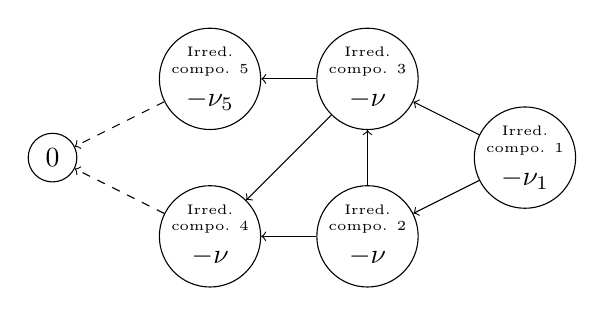
\begin{tikzpicture}
    \newcommand\component[4]{
      \node[circle,draw,minimum size=1cm,text width=1cm,inner
      sep=0pt,align=center] at (-#1,#2) (#3)
      {\tiny Irred.\\compo.~#3\par\normalsize$-\nu_{#4}$};
      %\node at (#1,#2+.3) {$\nu_{#3}$};
    }
    \component{0}{1}{1}{1};%
    \component{2}{0}{2}{{}};
    \component{2}{2}{3}{{}};
    \component{4}{0}{4}{{}};
    \component{4}{2}{5}{5};
    \node[circle,draw] at (-6,1) (0) {0};
    \draw[->] (1) edge (2) (1) edge (3) (2) edge (3)
    (3) edge(5) (3) edge (4) (2) edge (4) 
    (5) edge[dashed] (0) (4) edge[dashed] (0);% (3) edge[dashed] (0);
  \end{tikzpicture}
  \caption{Example of a communication graph over the irreducible
    components of a matrix $Q$. Each component $j$ has a maximal
    eigenvalue $-\nu_j$ that is simple. The dashed lines to $0$ are
    just a reminder that the sums over some lines in $Q$ are negative,
    corresponding to a transition to the absorbing state $(0)$ in
    matrix $P$.}
  \label{fig:irreducible}
\end{figure}

To illustrate this definition, let us consider the transition graph of
Figure~\ref{fig:irreducible} and assume that
$-\nu_2=-\nu_3 =-\nu_4=-\nu$ are maximal. The degree is $d=3$ because
the path
$Q_{1,1}\rightarrow Q_{2,2} \rightarrow Q_{3,3} \rightarrow Q_{4,4}$
contains 3 tagged components.





\subsection{Classical coupon collector and double-dixie problems.}
\label{ssec:classic}

As mentioned in the introduction, the coupon collector can be seen as
the simplest instance of our problem. Here, we use it as an illustration of
how to use Theorems~\ref{TH:GUMBEL} and \ref{TH:MOMENTS}.  It shows
the usefulness of our approach: the well-known formulas for the
classical coupon collector are obtained directly.


We consider the classical coupon collector problem: there are $n$
different types of coupon.  At each time step, a coupon of type $i$ is
picked at random, uniformly among all coupon types, until $k$ coupons
of each kind are collected.  It is proved in \cite{double-dixie} that
the expectation of $T_n$ (average time to collect $k$ coupon of each
type is bounded by $n(\log n + (k-1)\log\log n +O(1))$. In this
section, we show that our approach allows one to retrieve this result
directly and even get the more precise statement given in
\cite{Erdos}: We also provide the asymptotic distribution of $T_n$ and
the asymptotics of its moments.

At time $0$, all chains start in state $k$:
$\alpha=(0,\dots,0,1)$. The transition graph of each coupon type is
\begin{center}
  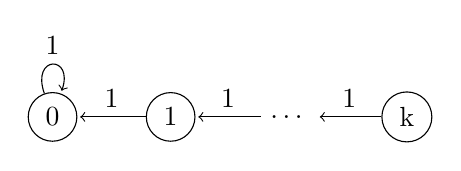
\begin{tikzpicture}[shorten >=1pt,xscale=1.5]
    \node[circle,draw] at (0,0) (0) {0};
    \node[circle,draw] at (1,0) (1) {1};
    \node at (2,0) (2) {\dots};
    \node[circle,draw] at (3,0) (k) {k};
    \draw (1) edge[->] node[above] {1} (0);
    \draw (2) edge[->] node[above] {1} (1);
    \draw (k) edge[->] node[above] {1} (2);
    \draw (0) edge[->,loop above] node[above] {1} (0);
  \end{tikzpicture}
\end{center}
This is certainly the simplest chain with an absorbing state and, in
isolation, the absorbing time for each component is trivial and is
equal to $k$.  This case is homogeneous (all coupon types have the
same transition matrix) and uniform (uniform choice among all coupon
types).

The matrix $Q$ (defined in \eqref{eq:defQ}) corresponding to this
Markov chain is a $k\times k$ matrix that has $-1$ on its diagonal and
$1$ on its sub-diagonal. It has one eigenvalue $-\nu=-1$ that has a
degree $k$.  In the homogeneous and uniform case, the
ODE~\eqref{eq:ode} becomes
\begin{equation*}
  \left\{
    \begin{array}{lcll}
      \displaystyle\frac{d}{dt}M_k(t)%
      &=& \displaystyle-\frac1nM_{k}(t) &\\[1em]
      \displaystyle\frac{d}{dt}M_i(t)%
      &=& \displaystyle-\frac1nM_{i}(t)+\frac1nM_{i+1}(t) & \quad \mathrm{for}~0<i<k
  \end{array}
  \right.
\end{equation*}
with $M_k(0)=1$ and $M_i(t)=0$ for $i\in\{0\dots k-1\}$.

$M_0(t)$ is the cumulative distribution function of an Erlang variable
of parameter $(k,1)$ (\emph{i.e.} the sum of $k$ \emph{i.i.d.}
exponential variables of parameter $1$) which can be written:
\begin{align*}
  M_0(t)&=1-\sum_{i=0}^{i-1}\frac{(t/n)^ie^{-t/n}}{i!}
          =1-\frac{(t/n)^{k-1}e^{-t/n}}{(k-1)!}+O((t/n)^{k-2}e^{-t/n}).
\end{align*}
The solution in $t$ of $\frac{(t/n)^{k-1}e^{-t/n}}{(k-1)!} = 1/n$ is
$-n(k-1)W_{-1}\left(\frac{-1}{k-1}\left(\frac{(k-1)!}{n}\right)^{1/n}
\right)$,
where $W_{-1}$ is the second branch of the Lambert $W$
function ($W_{-1}(z)$ is the unique solution of
$W_{-1}(ze^z)=z$ for $z \leq -1$).  Since
$W_{-1}(x) = \log(-x) - \log(-\log(-x)) + o(1)$ when $x<0$ approaches
$0$, one gets
$t_n=n (\log n + (k-1) \log\log n - \log((k-1)!))  + o(n)$.  Using
Theorems~\ref{TH:GUMBEL}, and \ref{TH:MOMENTS}, this shows that the
time $T_n$ to collect $k$ coupons of each type satisfies:
\begin{align*}
  \lim_{n\to\infty} & \proba{T_n\le n[\log n {+} (k-1)\log \log n 
    +x]}=e^{-\frac{e^{-x}}{(k-1)!}} \\
  \expect{T_n}&= n\log n {+} (k{-}1)n\log \log n 
    {+} n(\gamma{-}\log((k{-}1)!) +o(n) \\
 \variance{T_n} &= \frac{\pi^2n^2}{6 } + o(n^2).
\end{align*}
The first two results were first established in \cite{Erdos}. For the
special case $k=1$, a slightly stronger form of the third formula has
been proven is \cite{BRAYTON196331}, where the $o(n^2)$ is shown to be
$O(n^2\log\log\log n / \log\log n)$. In the case of general $k$, the
third formula had been conjectured in \cite{doumas2014coupon}.

It is interesting to 
notice  that the variance of $T_n$ does not depend on $k$ when $n$ is large, and more
generally  that the asymptotic distribution of $T_n$
is Gumbel and its shape does not depend on $k$.


To illustrate this result and give a grasp on the respective behaviors
of $T_n$ and $t_n$ with $n$, we ran several simulations of the coupon
collector (with $k=3$) and display the corresponding values of $T_n$
and $t_n$.  Figure~\ref{fig:simu_20-200} shows the empirical
proportion of coupons collected up to time $t$, $M_0(t)$ and its fluid
approximation $1-m(t)$ (using the notations of Section
\ref{ssec:defhomo}).  Although these plots only show a single
trajectory and its fluid limit, they are rather typical.  They
illustrate the fact that $T_n$ and $t_n$ are very close to each other.
\begin{figure}[ht]
  \centering
  \begin{tabular}{@{}c@{}c@{}c}
    \includegraphics[width=.38\linewidth]{simu_20.pdf}
    &\includegraphics[width=0.4\linewidth]{simu_200.pdf}
    &\includegraphics[width=0.22\linewidth]{simu_200_zoom.pdf}\\
    (a) $n=20$ &(b) $n=200$&(c) $n=200$ (zoom)
  \end{tabular}
  \caption{Illustration of the fraction of the $n$ coupons that have
    been collected $k=3$ times as a function of time.  We also compare
    the stochastic hitting time $T_n$ with the fluid approximation
    $t_n$ for $n=20$ and $n=200$. }
  \label{fig:simu_20-200}
\end{figure}




We have also computed the empirical distribution of $T_n$ and tested
it against its limit Gumbel distribution.  Figure~\ref{fig:db} shows
the cumulative empirical distribution of $T_n$ as well as the
cumulative distribution of a Gumbel distribution with different values
of $n$.  In the case $k=1$, the convergence appears to be quick and
the cumulative distribution of $(T_n-t_n)/n$ seems to coincide with
the one of the Gumbel distribution for $n\ge100$. For $k=5$, even if
one can convince oneself that there is convergence to the limit
distribution, this convergence appears to be slow.


\begin{figure}[ht]
  \centering
  \begin{tabular}{@{}cc@{}}
    \begin{tabular}{c}\includegraphics[width=.45\linewidth]{gumbel_k1}\end{tabular}
    &\begin{tabular}{c}\includegraphics[width=.45\linewidth]{gumbel_k5}\end{tabular}
    \\
    $k=1$ & $k=5$
  \end{tabular}
  \caption{Empirical cumulative distribution of $(T_n-t_n)/n$ and its
    limit Gumbel distribution. }
  \label{fig:db}
\end{figure}





\subsection{Numerical methods for $t_n$: an example with non-uniform
  probabilities.}
\label{sec:non_unif}

The case when probabilities to get the different coupons are not
uniform is also well studied (see for example \cite{Berenbrink} and
references therein).  Most papers provide bounds on the collection
time.  When the probability vector $(p_1, \dots , p_n)$ satisfy
Assumptions \eqref{eq:assum1} and \eqref{eq:assum2}),
Theorem~\ref{TH:MOMENTS} shows that
$\expect{T_n}= t_n + n\gamma/\nu + o(n)$, where $t_n$ satisfies
\begin{equation}
  \label{eq:non_unif_t_n}
  \sum_{i=1}^n \alpha \exp(p_iQt_n){\bf 1} = 1.
\end{equation}

There is in general no closed-form formula for $t_n$. Yet,
Equation~\eqref{eq:non_unif_t_n} is easy to solve numerically (using a
classical Newton's method for example) with a very good
precision. This can be done by using a numerical computation of the
exponential of the matrix $Q$.  Similarly, the value of the largest
eigenvalue of $Q$ can be computed numerically.  This numerical
computation provides an alternative method to estimate $T_n$, much
faster than the repetition of simulations.

We illustrate this method and show its accuracy by computing the time
to collect $k$ coupons that have non-uniform probabilities, under the
two following probability distributions, that we call $p^{\log}$ and
$p^{\text{square}}$. These distributions $p^{\log}$ and $p^{\text{square}}$ select the chain
$i$ with probabilities respectively proportional to
$(\log (1+i))^{-1}$ and $i^{-2}$. For a system with $n$ chains, these
probabilities are:
\begin{align*}
  p_i^{\log} &= \frac{(\log (1+i))^{-1}}{\sum_{j=1}^n (\log(1+j))^{-1}}\\
  p_i^{\text{square}} &= \frac{i^{-2}}{\sum_{j=1}^n j^{-2}}
\end{align*}

We implemented a simulator of the non-uniform coupon collector and a
numerical algorithm that computes the quantity $t_n+\gamma/p_n$. We
compare the value $\expect{T_n}$ (computed by averaging $1000$ runs of
the simulator) with the quantity $t_n+\gamma/p_n$. We report the
results in Table~\ref{tab:non_unif} for three different probability
distribution: uniform ($p_i=1/n$), log ($p_i\propto 1/\log(1+i)$) and
square ($p_i\propto 1/i^2$). We observe that in all cases, there is a
good match between the approximation and the simulation. Also, as
expected, the average hitting time $\expect{T_n}$ is the smallest for
the uniform distribution and is the largest for the square
distribution.

The time taken by our simulator to compute $1000$ simulations for
$n=50$ and $k=5$ is about ten minutes. In contrast, it takes less than
a second to compute the value $t_n$ with a non-optimize implementation
of the numerical algorithm that uses a dichotomic search and the
standard matrix exponential function of \texttt{python} \texttt{numpy}
to compute $t_n$. The most costly operation of our implementation is
the evaluation of the left hand side of
Equation~\eqref{eq:non_unif_t_n} that requires the computation of $n$
exponentials of $k\times k$ matrices. Moreover, by
Theorem~\ref{TH:MOMENTS}, the variance of the simulation for the
square distribution grows as $n^2$, which leads to confidence
intervals that grow with $n$. This makes the numerical computation of
$t_n$ much faster than the simulation for large values of $n$.

\begin{table}[ht]
  \centering
  \begin{tabular}{|c|l:c|l:c|l:c|}
    \hline
    &\multicolumn{2}{c|}{$n=10$}&
     \multicolumn{2}{c|}{$n=20$}&
     \multicolumn{2}{c|}{$n=50$}\\
    &Simulation & $t_n{+}\frac{\gamma}{p_n}$ &Simulation & $t_n{+}\frac{\gamma}{p_n}$ &Simulation & $t_n{+}\frac{\gamma}{p_n}$  \\
    \hline
    \hline
    Unif ($k=5$)& $29.4\pm0.2$&28.8&$71.8\pm0.5$&71.5&$224.2\pm1.2$&224.5\\
    \hline log
    ($k=1$)&$35.8\pm1.0$&35.9&$88.3\pm2.0$&90.2&$275.5\pm5.0$&277.6\\
    \hline square ($k=1$)&$247.6\pm9.3$&271.5&$1255\pm39$&1346&$10590\pm262$&10950\\
    \hline Unif ($k=5$)&$89.4\pm0.4$&85.7&$199.7\pm0.7$&194.6&$569.8\pm1.8$&557.9
    \\\hline log ($k=5$)&
                        $116.3\pm1.8$&109.9&$257.3\pm3.2$&251.1&$720.9\pm7.8$&704.0
    \\\hline square
    ($k=5$)&$922\pm18$&834.5&$4209\pm77$&3987&$31277\pm455$ & 30214\\
    \hline
  \end{tabular}
  \caption{Coupon collector and non-uniform probabilities: Comparison
    between the approximation $t_n+\gamma/p_n$ and the empirical average
    of $\expect{T_n}$ computed over $1000$ runs of the simulator.  The
    value $\pm x$ indicate the $95\%$ confidence intervals on the
    mean. } 
  \label{tab:non_unif}
\end{table}

\subsection{Bounding $T_n$ by using $T_1$:  Example
  of erasure channels.}
\label{sec:erasure}


The general formula for $t_n$ involves the largest eigenvalue of $Q$.
For the classical coupon collector, this eigenvalue is easy to compute
in closed form.  This is not true in general. As for non-uniform
probabilities, a numerical algorithm can always be used to compute
$t_n$. In this section, we provide an alternative by showing that an
upper bound on $t_n$ can be computed by using $T_1$, the hitting time
of $0$ for a single component. This quantity is often much easier to
compute.

We consider the system made of  a single component. The quantity
$\expect{T_1\mid X_1(0)=x}$ is the expected hitting time of $0$
starting from a state $x$. We define the quantity ${\bf T}_1^{\max}$ to be
the largest expected hitting time, over  all possible initial states $x$:
\begin{equation}
  {\bf T}_1^{\max}=\max_{x\in\{1\dots k\}}\expect{T_1 \mid X_1(0)=x}.
  \label{eq:T_1max}
\end{equation}
Our next result uses the fact that ${\bf T}_1^{\max}$ is an upper
bound on $-1/\nu$, with possible equality only if the degree is
one. It implies that in particular that the expectation of the hitting
time $T_n$ satisfies
\begin{equation}
  \expect{T_n}\le {\bf T}_1^{\max}(n\log n + n\gamma) + o(n). 
  \label{eq:absorbing_bound}
\end{equation} 
This inequality is most of the time strict. For example, for the
coupon collector with $k$ coupons, ${\bf T}_1^{\max}=k$ and
$t_n=n\log n + (k-1)n\log\log n +O(n) \ll kn\log n+O(n)$.  Also, the
inequality is in general strict, even when the matrix $Q$ is
irreducible. An example is the case of the erasure channel, shown in
this section: The upper bound reported in
Figure~\ref{fig:erasure_result} is strict while the original matrix
$Q$ is irreducible.
\begin{thm}
  \label{th:absorbing_bound}
  Let ${\bf T}_1^{\max}$ be defined as in
  Equation~\eqref{eq:T_1max}. Then, in the case of uniform probabilities
  $p_i=1/n$:
  \begin{align*}
    t_n \le {\bf T}_1^{\max} n \log n + o(n). 
  \end{align*}
\end{thm}


\begin{proof}
  Theorem~\ref{TH:MOMENTS} combined with Equation~\eqref{eq:tn}
  shows that
  $\expect{T_n}=(1/\nu)n\log n + ((d-1)/\nu) n \log \log n -
  n\log(a\nu^{1-d})/\nu + n\gamma/\nu + o(n)$,
  where $-\nu$ is the largest eigenvalue of $Q$ and $d$ is the degree
  of the eigenvalue $-\nu$. We now show that
  $1/\nu\le {\bf T}^{\max}_1$ with possible equality only in a special case, treated later.

  As $Q$ is non-singular, we have: 
  \begin{align*}
    \expect{T_1 \mid X_1(0)=x} %
    &= \sum_{t=0}^\infty \proba{T_1\ge t\mid X_1(0)=x}\\
    &=\sum_{t=0}^\infty \sum_{j=1}^k(I+Q)^t_{xj} =
      -\sum_{j=1}^k(Q^{-1})_{xj}. 
  \end{align*}
  The largest eigenvalue of $Q^{-1}$ is $-1/\nu$. Moreover, the term
  $Q^{-1}_{xj}$ is a sum of non-negative terms and is therefore
  non-negative. By Perron-Frobenius theorem, this implies that
  $-1/\nu\le \max_{x} \sum_j -Q^{-1}_{xj} = {\bf T}_1^{\max}$.

If the inequality is strict, we get the desired result, namely  $t_n \le {\bf T}_1^{\max} n \log n + o(n)$.

Now, the inequality becomes  an equality only when the eigenvalue  $-1/\nu$ of    $Q^{-1}$ admits $\mathbf{1}$ as an eigenvector.
This implies that $\exp(Qt)$ also admits  $\mathbf{1}$ as an eigenvector for eigenvalue $\exp(-\nu t)$.
In this case,  the quantity $ \alpha \exp(Qt)\mathbf{1}$ used in the definition of $t_n$  can be computed exactly and is equal to  $\alpha \exp(-\nu t)\mathbf{1} =  \exp(-\nu t)$, because $\alpha \mathbf{1} = 1$.
Therefore $t_n$ admits an exact form,  $  t_n = \frac{1}{\nu} n \log n =  {\bf T}_1^{\max} n \log n$.



  
\end{proof}

Let us illustrate this theorem with the following chain for each
component:

\begin{center}
  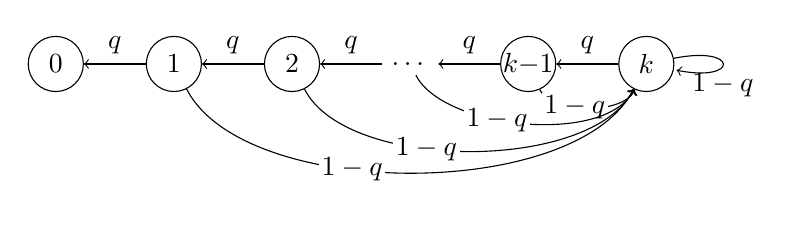
\begin{tikzpicture}[xscale=1.5]
    \tikzstyle{state}=[circle,draw,inner sep=0pt,minimum width=0.7cm]
    \foreach \i in {0,1,2} {\node[state] at (-5+\i,0) (\i) {\i};}
    \node at (-2,0) (3) {\dots};
    \node[state] at (-1,0) (k-1) {$k{-}1$};
    \node[state] at (0,0) (k) {$k$};
    \foreach \i/\j in {k/k-1,k-1/3,3/2,2/1}{
      \draw (\i) edge[->] node[above]{$q$} (\j);
      \draw (\j) edge[->,in=-110,out=-70] 
      node[fill=white,inner sep=1pt,pos=.4]{$1-q$} (k);
    }
    \draw (1) edge[->] node[above]{$q$} (0);
    \draw (k) edge[->,loop right] node[below]{$1-q$}(k);
  \end{tikzpicture}
\end{center}
This is a natural model of the lifetime of an {\it erasure channel }
system.  An erasure channel transmits bits and each of them gets
erased with probability $p$.  The state of the channel is the current
number of consecutive bits that have been erased.  When this number
reaches some value $k$ (that depends on the forward error correction
that is used), the message transmitted on the channel cannot be
corrected anymore and the channel is declared faulty.  Here we
consider a communication system made of $n$ parallel independent
erasure channels and we look at its lifetime: When all channels become
faulty, the communication stops.

For this example, the quantity ${\bf T}^{\max}_1$ can be easily
computed in closed form.  Indeed, let
$h_j:=\expect{T_1 \mid X_1(0) = j}$ be the expected hitting time of
$0$ starting from $j$. We have $h_0=0$ and for $j\in\{1,\dots,k\}$:
\begin{equation*}
  h_j = 1+q h_{j-1} + (1-q) h_k.
\end{equation*}
One can verify that the vector $h$ such that
$h_j=\sum_{i=0}^{j-1} q^{i-k}$ is the unique solution of the above
system of equations. This implies that
${\bf T}^{\max}_1=\max_{j\in\{0,\dots,d\}}h_j = \sum_{i=0}^{k-1}
q^{i-k}=(q^{-k}-1)/(1-q)$.
Hence, Theorem~\ref{th:absorbing_bound} implies that for this example:
\begin{equation}
  \label{eq:absorbing_bound_ex}
  \expect{T_n} \le \frac{q^{-k}-1}{(1-q)}(n\log n + \gamma) + o(n).
\end{equation}

We implemented a simulator of the erasure model as well as a numerical
algorithm to compute the asymptotically exact approximation
$t_n+n\gamma/\nu$. We restrict our comparison to the case of uniform
probabilities.  To compute numerically $t_n$, we use a dichotomic
algorithm similar to the one of Section~\ref{sec:non_unif} and we use
functions from \texttt{numpy} standard library to compute the
eigenvalue $-\nu$.  In Figure~\ref{fig:erasure_result}, we compare
numerically the bound provided by
Equation~\eqref{eq:absorbing_bound_ex}, with the asymptotically exact
bound of Theorem~\ref{TH:MOMENTS}. We report the results for
$n=10$. We also computed the results for larger values of $n$. They
are similar and not reported in the paper.

\begin{figure}[ht]
  \centering
  \includegraphics[width=.6\linewidth]{erasure_channel}
  \caption{Erasure channel: Comparison of an estimation of
    $\expect{T_n}$ computed by simulation, the asymptotic result of
    Theorem~\ref{TH:MOMENTS} and the upper bound of
    Theorem~\ref{th:absorbing_bound} as a function of the success
    probability $p$. The simulation results are averages over $10^4$
    values. The confidence intervals on the mean are plotted on the
    figure but they are too small to be visible. }
  \label{fig:erasure_result}
\end{figure}

We observe that, for this model, the approximation $t_n+n\gamma/\nu$
is very close to the value obtained by simulation, even when
$n=10$. Second, as expected, $T^{\max}_1(n\log n+\gamma)$ is an upper
bound on this value. For large values of $q$, this upper bound is loose
(roughly twice as large as  $t_n+n\gamma/\nu$). This bound becomes
tighter as $q$ decreases (about $3\%$ off the correct value when
$q=0.7$).


\section{Coupling  time of random walks.}
\label{sec:rw}


In general, computing 
coupling times of Markov chains is  useful because they provide
bounds on their mixing times,
\cite{peres}. They also correspond to the average time complexity of perfect simulation algorithms \cite{PW96}.
As for random walks, they are often used to model discrete event
systems, such as queuing networks.
Here we consider a random walk on a finite grid $\{1,\dots,k\}^n$.
 We first analyze a non-lazy random walk. It is usually more difficult to
deal with coupling times in non-lazy random walks, while it makes no
difference with our approach.

The random walk is defined as follows. 
From a position $(x_1,\ldots,x_i,\ldots,x_n)$ the walker moves to a
neighboring position $(x_1,\ldots,x_i+1, \ldots, x_n)$ with
probability $q_i$ and to $(x_1,\ldots,x_i-1 , \ldots, x_n)$ with
probability $r_i$.  On the boundaries, with probability $q_i$
(resp. $r_i$) the walker remains at the same position if $x_i = k$
(resp. $x_i = 1$). In the following we will consider several possible
values of $(q_i)$ and $(r_i)$ satisfying assumptions \eqref{eq:assum1}
and \eqref{eq:assum2}.  The random walk in dimension two is displayed
in Figure~\ref{fig:rw2}.

\begin{figure}[hbtp]
  \centering
  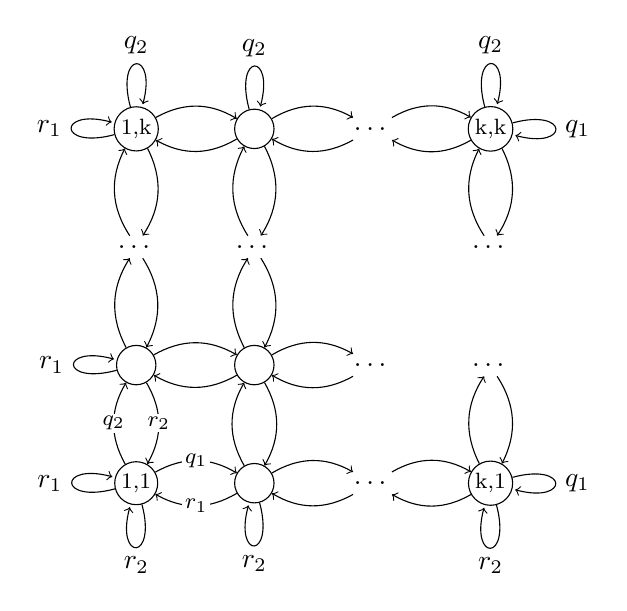
\begin{tikzpicture}[scale=1.5]
    \newcommand\lien[2]{\draw (#1) edge[e] (#2) (#2) edge[e] (#1);}
    \newcommand\lienP[3]{\draw (#1) edge[e] node[ne]{\footnotesize $q_{#3}$} (#2) 
                         (#2) edge[e] node[ne]{\footnotesize $r_{#3}$} (#1);}
    \tikzstyle{state}=[circle,draw,inner sep=1pt,minimum width=.5cm]
    \tikzstyle{ne}=[inner sep=1pt,fill=white]
    \tikzstyle{e}=[bend left,->]
    \node[state] at (2,4) (2k) {};
    \node[state] at (4,4) (kk) {\footnotesize k,k};
    \node[state] at (1,1) (11) {\footnotesize 1,1};
    \node[state] at (1,2) (12) {};
    \node[state] at (2,1) (21) {};
    \node[state] at (2,2) (22) {};
    \node[state] at (1,4) (1k) {\footnotesize 1,k};
    \node[state] at (4,1) (k1) {\footnotesize k,1};
    \node        at (3,1) (d1) {\dots};
    \node        at (3,4) (dk) {\dots};
    \node        at (1,3) (1d) {\dots};
    \node        at (2,3) (2d) {\dots};
    \node        at (4,2) (k2) {\dots};
    \node        at (4,3) (k3) {\dots};
    \node        at (3,2) (d2) {\dots};
    \draw (1k) edge[loop above] node{$q_2$} (1k); 
    \draw (2k) edge[loop above] node{$q_2$} (2k); 
    \draw (kk) edge[loop above] node{$q_2$} (kk); 
    \draw (11) edge[loop below] node{$r_2$} (kk); 
    \draw (21) edge[loop below] node{$r_2$} (kk); 
    \draw (k1) edge[loop below] node{$r_2$} (kk); 
    \draw (11) edge[loop left] node{$r_1$} (kk); 
    \draw (12) edge[loop left] node{$r_1$} (kk); 
    \draw (1k) edge[loop left] node{$r_1$} (kk); 
    \draw (kk) edge[loop right] node{$q_1$} (kk); 
    \draw (k1) edge[loop right] node{$q_1$} (kk); 
    \lienP{11}{21}{1}\lienP{11}{12}{2} % lien avec proba de transition 
    \lien{21}{d1}\lien{d1}{k1}\lien{12}{22}\lien{22}{2d} % liens seuls
    \lien{12}{1d}\lien{1d}{1k}\lien{21}{22}\lien{2d}{2k}\lien{22}{d2} % liens seuls
    \lien{1k}{2k}\lien{2k}{dk}\lien{dk}{kk}\lien{k1}{k2}\lien{k3}{kk} % liens seuls
  \end{tikzpicture}
  \caption{Random walk in two dimensions with borders.}
  \label{fig:rw2}
\end{figure}




We consider a coupling of $k^n$ versions $({\bf X}_{x})_{x \in \{1 \dots
  k\}^n}$, of the chain ${\bf X}$, one per possible initial state,  under which
all chains take the same transitions. We are interested in computing
the first time $T_n$ such that the state of the system does not depend
on the initial state, \emph{i.e.}, such that for any initial state
$x$ and $y$: ${\bf X}_{x}(T_n)= {\bf X}_{y}(T_n)$ (note that by assumption
on the coupling, this implies that  ${\bf X}_{x}(t)= {\bf X}_{y}(t)$ for $t\ge T_n$).

By monotonocity of the random walk, the coupling time $T_n$ is equal
to the coupling time of the two extreme chains ${\bf L}$ and ${\bf U}$ starting
respectively in the extreme points, namely ${\bf L}(0) = (1,\dots,1)$ and
${\bf U}(0) = (k,\dots,k)$.  Another property of this coupling is that
whenever coalescence occurs in one coordinate, say $i$,
($L_i(t_0) = U_i(t_0)$) then this partial coalescence remains:
$\forall t \ge t_0$, $L_i(t) = U_i(t)$.


We consider the Markov chain $\bf X \bydef ({\bf L,U})$.  Each component,
corresponding to one coordinate, $X_i := (L_i,U_i)$, is selected with
probability $p_i := q_i + r_i $.  Once a coordinate has been chosen,
the two walks $U_i$ and $L_i$ take the same step: They both increase
(resp. decrease) their $i$-th coordinate with probability $q_i/p_i$
(resp. $r_i/p_i$), if possible.  Each component has two absorbing states
corresponding to the coalescence of $L_i$ and $U_i$, namely $(1,1)$
and $(k,k)$.  Note that it makes no difference with the case with a
single absorbing state because one can always merge all absorbing
states into one.

All this implies that this chain fits in our general framework by using the
transition matrix for each component depicted in Figure~\ref{fig:rw1}.
At time $0$, the difference is maximum: $(L_i(0),U_i(0))=(1,k)$.  If
the chain is a state $(a,b)$ (with $a<b$), it jumps to the state
$(a+1,\min(b+1,k))$ with probability $q_i/p_i$ and to the state
$(\max(a-1,0),b-1)$ with probability $1-q_i/p_i$. 


\begin{figure}[hbtp]
  \centering
\includegraphics[width=0.65\textwidth]{transMartrxRW.fig}
\caption{transition matrix of the chain $X_i = (L_i,U_i)$}
\label{fig:rw1}
\end{figure}





\subsection{Homogeneous and uniform case.}
Let us first consider the homogeneous and uniform case.  In our
context, this means that $q_i$ and $r_i$ do not depend on $i$.  Of
course this implies that $p_i = q_i+ r_i = 1/n$.  However homogeneity
and uniformity do not imply that $q_i = r_i$. Therefore, the walk can
still have a drift.  In the rest of this subsection, the index $i$ is
useless and will be dropped.

The asymptotics of $T_n$ depend on the largest eigenvalue of $Q$.  As
seen in Figure~\ref{fig:rw1}, this matrix is block lower triangular
because the difference $U - L$ cannot increase.  Therefore, the
largest eigenvalue of $Q$ is the largest eigenvalue of one of its
block diagonal matrices.  It should be clear that the block with the
largest eigenvalue is the  largest block, corresponding to the
level $U_i - L_i = 1$ in Figure~\ref{fig:rw1}.  The sub-matrix of $Q$
corresponding to this $(k-1)\times (k-1)$ block is
\begin{equation}
  {A} = %
  \begin{bmatrix}%
    -(c+d) & c & & & \\ %
    d & -(c+d) & c & & & \\ %
    & d & \ddots & \ddots &\\
     & & \ddots & \ddots & c\\
     &  & & d & -(c+d)
  \end{bmatrix},
\label{eq:block}
\end{equation}
with $c=nq$ and $d=nr$.


It is shown in \cite{kulkarni1999eigenvalues} that the eigenvalues of
this matrix are
$-(d+c)+2\sqrt{cd}\cos(j\pi/k) = -1+2\sqrt{n^2qr}\cos(j\pi/k), \quad j \in \{1,\ldots,k\}$.
Hence, the eigenvalue with the largest real part is
$-1+2n\sqrt{qr}\cos(\pi/k)$ and its  multiplicity is $1$.
\begin{itemize}
\item When $p \not=q$, Theorem~\ref{TH:MOMENTS}, together with
  $\cos(\pi/k)\le1$, imply that the coupling time $T_n$ satisfies
  \begin{align*}
    \expect{T_n} & =   \frac{1}{1-2n\sqrt{qr}\cos(\pi/k)}n\log n +
                   O(n)\\
                 & \lesssim  \frac{1}{1-2\sqrt{cd}} n \log n + O(n),
  \end{align*}
  where $c \bydef nq$ and $d \bydef nr$ are the normalized
  probabilities that do not depend on $n$.  Note that the
  approximation $\cos(\pi/k)\approx1$ becomes more accurate as $k$
  grows.
  
\item The case $q=r=\frac{1}{2n}$ corresponds to the random walk with
  no drift.  In this case one can use the second order Taylor
  expansion $1-\cos(\pi/k)\approx\pi^2/(2k^2)$.  This implies
  \begin{align*}
    \expect{T_n} & =   \frac{1}{1-\cos\p{\frac{\pi}{k}}}n\log n + O(n) \\
                 &\approx \frac{2k^2}{\pi^2} n\log n + O(n).
  \end{align*}
\end{itemize}

At this point, one can notice that this approach provides an
equivalent to the coupling time rather than an upper bound, as usually
done in the literature \cite{peres}.  Also note that the asymptotic
behavior of the random walk with a drift is very different from the
case with no drift: in the drift case, the asymptotic coupling time
does not depend on $k$, the size of the grid, while in the no-drift
case, the coupling time grows as $k^2$.



\subsection{Heterogeneous cases.}

We first consider the heterogeneous case with uniform choices,
\emph{i.e.}, $q_i+ r_i = 1/n$ so that the coordinate $i$ is chosen
with probability $1/n$.  To comply with conditions \eqref{eq:assum1}
and \eqref{eq:assum2}, and with the assumptions of Theorem
\ref{TH:HETERO}, we assume that $q_i$ is of the form $c_i/n$ for all
$i$ (where $c_i$ is a constant).  Uniformity implies that
$r_i = (1-c_i)/n$.


By applying the results of Theorem \ref{TH:HETERO} and the general
form of the eigenvalues of the matrix of Equation~\eqref{eq:block},
there exists $\bar{c}\in [\min c_i,\max c_i]$ such that the coupling
time is:
\begin{equation*}
  \expect{T_n} =   \frac{1}{1-2\sqrt{\bar{c}(1-\bar{c})}\cos\p{\frac{\pi}{k}}} n\log n +
  O(n). 
\end{equation*}

Let us now consider a random walk with heterogeneous as well as
non-uniform transitions.  This is the case when, for example, for all
$i$, $p_i =c_i/n$ and $q_i = d_i/n$ but $c_i+d_i$ is not necessarily
equal to $1$.  In that case, Theorem \ref{TH:HETERO} says that there
exist $\bar{c}\in[\min c_i,\max c_i]$ and
$\bar{d}\in[\min d_i,\max d_i]$ such that the coupling time is:
\begin{equation*}
  \expect{T_n} = \frac{1}{\bar{d}+\bar{c}-2\sqrt{\bar{c}\bar{d}}\cos\p{\frac{\pi}{k}}} n\log n +
  O(n). 
\end{equation*}

This result calls for several comments.
\begin{itemize}
\item First, the behavior of the heterogeneous and/or non-uniform case
  is very similar to the homogeneous and uniform random walk with a
  drift: when $n$ is large: $\expect{T_n} \approx C n\log n$ where $C$
  is a constant that does not depend on $k$, the size of the state
  space.
\item Up to our knowledge, this is the first time an asymptotic of the
  coupling of a random walk with general probabilities (not dependent
  on the position) is computed in closed form.
\end{itemize}


\subsection{Lazy random walk on the torus.}

Other random walks can be analyzed with this approach. In this
section, we compute the coupling time of the uniform lazy chain on the
torus $\{0\dots k-1\}^n \mod (k,\dots,k)$, analyzed in Chapter 5 of
\cite{peres}. At each step, the lazy random walk remains at its
current position with probability $1/2$. With probability $1/2$, one
coordinate $i$ is picked and $X_i(t+1) = X_i(t)+1$, or $X_i(t)-1$,  with probability
$1/2$.  We show that the coupling time of the lazy chain is similar to
 the previous one.

We consider the following coupling of two lazy random walks $\bf X$ and
$\bf Y$ that start at $x$ and $y$ respectively. At each step, we first pick one of
the $n$ coordinates at random. If the positions of the two walks agree
in the chosen coordinate, we move both of the walks by $+1, -1$ or $0$
in that coordinate, with respective probabilities $1/4, 1/4$ and
$1/2$. If the positions of the two walks differ in the chosen
coordinate, we randomly choose one of the chains to move, leaving the
other fixed. We then move the selected walk by $+1$ or $-1$ in the
chosen coordinate, with probability $1/2$.

The coupling time of the chain is the first time when $\bf X$ and $\bf Y$ agree in
all coordinates.  For each coordinate, the clockwise difference
$\min \{ (X_i - Y_i) \mod k, (Y_i - X_i) \mod k \}$ has the transition
matrix displayed in Figure~\ref{fig:lazy}.


\begin{figure}[hbtp]
  \centering
  \begin{tabular}{c@{\hspace{1cm}}c}
    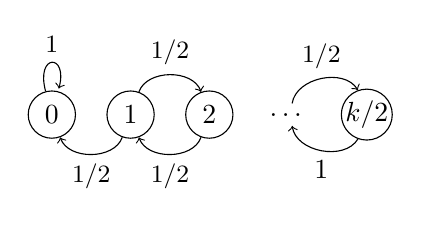
\begin{tikzpicture}[xscale=1]
      \tikzstyle{state}=[circle,draw,inner sep=0pt,minimum width=0.6cm]
      \foreach \i in {0,1,2} {\node[state] at (-5+\i,0) (\i) {\i};}
      \node at (-2,0) (3) {\dots};
      \node[state] at (-1,0) (k) {$k/2$};
      \foreach \i/\j in {2/1}{
        \draw (\i) edge[->,bend left,in=110,out=70] node[below]{\small $1/2$} (\j);
        \draw (\j) edge[->,bend left,in=110,out=70] 
        node[above]{\small $1/2$} (\i);
      }
      \draw (1) edge[->,bend left,in=110,out=70] node[below]{\small $1/2$} (0);
      \draw (k) edge[->,bend left,in=110,out=70] node[below]{$1$} (3);
      \draw (3) edge[->,bend left,in=110,out=70] node[above]{\small $1/2$} (k);
      \draw (0) edge[->,loop above] node[above]{\small $1$}(0);
    \end{tikzpicture}
    &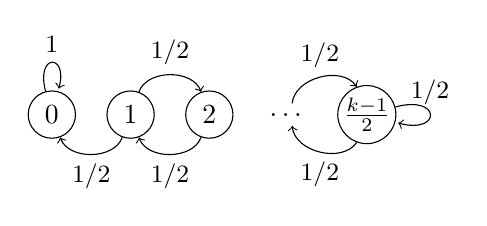
\begin{tikzpicture}[xscale=1]
      \tikzstyle{state}=[circle,draw,inner sep=0pt,minimum width=0.6cm]
      \foreach \i in {0,1,2} {\node[state] at (-5+\i,0) (\i) {\i};}
      \node at (-2,0) (3) {\dots};
      \node[state] at (-1,0) (k) {$\frac{k-1}{2}$};
      \foreach \i/\j in {k/3,2/1}{
        \draw (\i) edge[->,bend left,in=110,out=70] node[below]{\small $1/2$} (\j);
        \draw (\j) edge[->,bend left,in=110,out=70] 
        node[above]{\small $1/2$} (\i);
      }
      \draw (1) edge[->,bend left,in=110,out=70] node[below]{\small $1/2$} (0);
      \draw (k) edge[->,loop right] node[above]{\small $1/2$}(k);
      \draw (0) edge[->,loop above] node[above]{\small $1$}(0);
    \end{tikzpicture}
  \end{tabular}
  \caption{transition matrix of the chain
    $\min \{ (X_i - Y_i) \mod k, (Y_i - X_i) \mod k \}$. The cases
    when $k$ is even (left) and $k$ is odd (right) are different.
    However, they both correspond to the transition matrix $A$ folded
    in two.}
\label{fig:lazy}
\end{figure}

This transition matrix is the same as $A$, the largest diagonal block
of the previous chain, given in \eqref{eq:block}, but with size $k$
instead of $k-1$, and folded in two by the middle.
Therefore, the coupling time of the lazy walk   on the torus  is
asymptotically the same:

\begin{align*}
\expect{T_n} & =   \frac{1}{1-\cos\p{\frac{\pi}{k+1}}}n\log n + O(n) 
  \approx \frac{2(k+1)^2}{\pi^2} n\log n + O(n).
\end{align*}

This is a more precise statement than the results given in
\cite{peres} that only give bounds.


\section{Conclusions and Future work.}
\label{sec:conclusion}

In this paper, we have shown how fluid approximations can be used to
get precise and efficient estimations of the absorbing time of
discrete time Markov chains made of several components. Our approach
allows us to obtain closed form results or numerical methods that have
shown to be accurate as the number of chains $n$ goes to infinity.
We applied this approach to get closed form formulas for the coupon
collector, the lifetime of erasure channels and coupling times in
finite random walks.


One of the main features of our model is the fact that the components are
independent of each other (up to the mutual exclusion).  One could
think of extending our approach to interacting components, with
transition matrices that depend on the state of other components.  We
believe that the absorbing time of all the components can still be
computed using a similar approach.  One natural application of this
would be the computation of the time of extinction in several population dynamics
problems.
 
\subsection*{Acknowledgements}
We would like to thank Agn\`es Coquio who suggested the use of Poissonization 
and carefully read a preliminary version of this paper.

This project was partially supported by the EU project QUANTICOL
600708. 

\appendix

\section{Proof of Theorem \protect{\ref{TH:GUMBEL}}}
\label{sec:proof1}


We use the notations introduced in the paper before Theorem
\ref{TH:GUMBEL}, without recalling them here.  Note that to ease the
notations, we avoid to write explicitly the dependence of $p$ on $n$
and write $(p_1\dots p_n)$ instead of $(p^{(n)}_1\dots p^{(n)}_n)$.

  
  For a fixed $n$, the distribution $p_i$ satisfies
  $p_1\ge p_2\dots \ge p_n$. Let $f(t)=\alpha\exp(Qt)\mathbf{1}$. The
  function $f$ is non-increasing and positive. Hence, for all $\ell$, by
  definition of $t_n$ in Equation~\eqref{eq:t_n}, we have:
  \begin{align*}
    1 &= \sum_{i=1}^n f(p_it_n) \ge \sum_{i=n-\ell+1}^n f(p_it_n) \ge
        \ell f(p_{n-\ell}t_n).
  \end{align*}
  This shows that for all $\ell$, $f(p_{n-\ell}t_n)\le 1/\ell$.  By
  Assumption~\eqref{eq:assum2}, the quantity $p_{n-\ell}/p_n$
  converges to $1$ as $n$ goes to infinity. This implies that
  $f(p_{n}t_n)$ converges to $0$ and therefore that $p_nt_n$ converges
  to infinity as $n$ grows.
  Moreover, by
  Equation~\eqref{eq:density_f}, there exists a constant $a$ and an
  integer $d\ge1$ such that 
  \begin{equation}
    \label{eq:density_f_proof}
    f(t)=at^{d-1}e^{-\nu t}(1+O(t^{-1})).
  \end{equation}
  Let $\tilde g_n(x) = \proba{\widetilde{T}_n\le t_n+x/p_n}$.
  $\tilde{T}_n$ is the maximum of independent variables. Hence
  \begin{align*}
    \log(\tilde g_n(x)) &= \log \prod_{i=1}^n (1-f(p_i(t_n+x/p_n)))
                         = \sum_{i=1}^n
           \log(1- f(p_i(t_n+x/p_n))).
  \end{align*}
  By using $-\log(1-s)=s+o_{s\to0}(s)$ and
  Equation~\eqref{eq:density_f_proof}, we have:
  \begin{align}
    -\log \tilde g_n(x) 
    &= \sum_{i=1}^n f(p_i(t_n+x/p_n)) + o(1)\nonumber\\
    &= a\sum_{i=1}^n  (p_{i} (t_n+\frac{x}{p_n}))^{d-1} e^{-\nu
      p_i(t_n+\frac{x}{p_n})} + o(1)\nonumber\\
    &= a\sum_{i=1}^n (p_it_n)^{d-1} e^{-\nu p_i
      (t_n+\frac{x}{p_n})}(1+\frac{x}{t_np_n})^{d-1} + o(1)\nonumber\\
    &= a\sum_{i=1}^n (p_it_n)^{d-1} e^{-\nu p_i t_n} e^{-\nu x\frac{p_i}{p_n}}
      + o(1).
      \label{eq:g_tilde}
  \end{align}
  Assume that $x\ge0$.  The proof for $x\le0$ is similar, by
  inverting most of the signs ``$\ge$'' and ``$\le$''.
  As $p_i\ge p_n$, we have $e^{-\nu x p_i /p_n} \le e^{-\nu x}$.
  
  By definition of $t_n$ and Equation~\eqref{eq:density_f_proof}, we
  have $a\sum_{i=1}^n (p_it_n)^{d-1} e^{-\nu p_it_n}=1+o(1)$. This
  implies
  \begin{align*}
    -\log \tilde g_n(x) 
      &\le 
        e^{-\nu x}+o(1). 
  \end{align*}
  Let $\varepsilon>0$. Let $\ell_n$ be such that
  $p_{i}/p_n\ge(1+\varepsilon)$ if and only if $i\le n-\ell_n$ (which
  implies that $e^{-\nu x p_i/p_n}\ge e^{-\nu x (1+\varepsilon)}$ for
  $i\ge\ell_n$).  The sum in Equation~\eqref{eq:g_tilde} is greater
  than the sum of the last $\ell_n$ terms. Hence:
  \begin{align}
    - \log \tilde g_n(x) 
    &\ge a\sum_{i=n-\ell_n+1}^{n} (p_it_n)^{d-1} e^{-\nu
      p_i(t_n+\frac{x}{p_n})}+o(1)\nonumber\\ 
    & = a\sum_{i=n-\ell_n+1}^{n} (p_it_n)^{d-1} e^{-\nu
      p_it_n}e^{-\nu x \frac{p_i}{p_n}}  +o(1)\nonumber\\
    &\ge a\sum_{i=n-\ell_n+1}^{n} (p_it_n)^{d-1} e^{-\nu
      p_it_n}e^{-\nu x (1+\varepsilon)}  +o(1)\nonumber\\
    &= e^{-\nu x (1+\varepsilon)} -  e^{-\nu x (1+\varepsilon)}
      a\sum_{i=1}^{n-\ell_n} (p_it_n)^{d-1} e^{-\nu p_it_n} +o(1)
      \label{eq:g_tilde2}
  \end{align}
  where the last equality comes from the definition of $t_n$. 
  
  Therefore, to show the result, it suffices to show that the second
  term in Equation~\eqref{eq:g_tilde2} converges to $0$ as $n$ grows.
  By Assumption~\eqref{eq:assum1} and the definition of $\ell_n$, we
  have $p_{i-\ell_n}/p_i\ge p_{n-\ell_n}/p_n
  \ge1+\varepsilon$.
  Moreover, as $p_it_n$ converges to infinity, we have
  $(\frac{p_{i-\ell_n}}{p_i})^{d-1} e^{-\nu t_n(p_{i-\ell_n}-p_i)}\le
  (1+\varepsilon)^{d-1}e^{-\nu t_np_n\varepsilon}$.
  Hence, the last factor of the second term of
  Equation~\eqref{eq:g_tilde2} is:
    \begin{align*}
    a\sum_{i=1}^{n-\ell_n} (p_it_n)^{d-1} e^{-\nu p_it_n} 
    &= a\sum_{i=\ell_n}^{n} (p_{i-\ell_n}t_n)^{d-1} e^{-\nu p_{i-\ell_n}t_n}\\
    &\le a\sum_{i=\ell_n}^{n} (p_it_n)^{d-1} e^{-\nu p_it_n}
      (1+\varepsilon)e^{-\nu t_np_n\varepsilon}\\
    &\le a\sum_{i=1}^{n} (p_it_n)^{d-1} e^{-\nu p_it_n}
      (1+\varepsilon)e^{-\nu t_np_n\varepsilon}\\
    &= (1+\varepsilon)e^{-\nu t_np_n\varepsilon} + o(1). 
  \end{align*}
  that converges to $0$ as $n$ goes to infinity.  

  The proof for $x\le0$ is similar, by inverting most of the
  signs ``$\ge$'' and ``$\le$''.

  \medskip We conclude by showing that $T_n$ and $\tilde T_n$ are
  close (in probability). Indeed, as mentioned in
  Section~\ref{ssec:poisson}, $\tilde T_n=Z_{T_n}$, where
  $Z_{k}=\sum_{i=1}^kE_i$ and $E_i$ are \emph{i.i.d} exponential
  random variable of mean $1$.  Applying Chebyshev's inequality shows
  that for all $c>0$,
  $\proba{\abs{Z_k-k}\ge c}\le \var[Z_k]/c^2=k/c^2$. 
By conditioning on $T_n$, and using $\expect{T_n}=\expect{\tilde T_n}$, this implies that 
  $\proba{\abs{\tilde{T}_n-T_n}\ge c}\le \expect{T_n}/c^2 = \expect{\tilde T_n}/c^2$.

  Let $\varepsilon>0$. Applying the previous bound with
  $c=\varepsilon/p_n$ shows that:
  \begin{align*}
    \proba{\tilde T_n\le t_n + \frac{x{-}\varepsilon}{p_n}}
    - \frac{p_n^2\expect{\tilde T_n}}{\varepsilon^2}
    \le\proba{T_n\le t_n + \frac{x}{p_n}}
    \le\proba{\tilde T_n\le t_n + \frac{x{+}\varepsilon}{p_n}}
    + \frac{p_n^2\expect{\tilde T_n}}{\varepsilon^2}
  \end{align*}
  In Step~2 of the proof of Theorem~\ref{TH:MOMENTS}\footnote{Note
    that Step~1 and Step~2 of the proof of Theorem~\ref{TH:MOMENTS}
    concern the convergence of $\tilde T_n$ and do not use that $T_n$
    is close to $\tilde T_n$.}, we show that
  $\expect{\tilde T_n}=t_n + O(1)$. This means that it suffices to
  shows that $\lim_{n\to\infty}(p_n)^2t_n=0$ to show the result.
  
  To show this, we first remark that for any $x\ge0$ and $\alpha\ge1$,
  we have 
  $e^{-\alpha x}\le \alpha e^{-x}$. Hence, using
  Equation~\eqref{eq:density_f_proof} and the fact that $p_nt_n$
  converges to infinity, we have $f(t_np_i)\le (p_i/p_n)f(t_np_n)$ for
  $n$ large enough. This implies that 
  \begin{align*}
    1=\sum_{i=1}^n f(t_np_i) \le \sum_{i=1}^n \frac{p_i}{p_n}
    f(t_np_n) = \frac{1}{p_n}f(t_np_n). 
  \end{align*}
  Similarly to Equation~\eqref{eq:tn},
  Equation~\eqref{eq:density_f_proof} implies that
  $t_n \le \frac{1}{\nu p_n}(\frac1{p_n}+(d-1)\log\log
  \frac1{p_n})+O(1/p_n)$.
  This in particular implies that $\lim_{n\to\infty}t_n(p_n)^2=0$.

  \section{Proof of Theorem \protect{\ref{TH:MOMENTS}}}
  \label{sec:proof2}
  
  The proof consists of three steps. We first obtain uniform upper and
  lower bounds on $g_n(x):=\proba{\tilde{T_n}\le t_n+x/p_n}$ on the
  intervals $[-p_nt_n/2;0]$ and $[0;+\infty)$. We then use these
  bounds to show that for all $m\in\{1,2\dots\}$, the sequence
  $[p_n(\tilde T_n-t_n)]^m$ is uniformly integrable, which shows that
  the moments of $p_n(\tilde T_n-t_n)$ converge to the one of a Gumbel
  distribution. Finally, we show that the moments of $p_n(T_n-t_n)$
  converge to the ones of $p_n(\tilde T_n-t_n)$.

  \textbf{Step 1}. Recall that
  $f(t)=at^{d-1}e^{-\nu t}(1+\epsilon(t))$ with
  $\lim_{t\to\infty}\epsilon(t)=0$. By definition of $t_n$, this
  implies
  $1=\sum_{i=1}^n f(p_it_n)=\sum_{i=1}^n a (p_it_n)^{d-1}e^{-\nu p_i
    t_n} (1+\varepsilon(p_it_n))$.
  As $p_i\ge p_n$ and $\lim_{n\to\infty}p_nt_n=\infty$, this implies
  that
  \begin{equation*}
    \sum_{i=1}^n a (p_it_n)^{d-1}e^{-\nu p_i t_n}=1+\varepsilon_n,
  \end{equation*}
  with $\lim_{n\to\infty}\varepsilon_n=0$.

  Moreover, for $x\in[0;p_nt_n/2]$, we have:
  \begin{align*}
    f(p_i(t_n-x/p_n))%\\
    % 
 &=a(p_i(t_n-x/p_n)^{d-1})e^{-\nu p_i(t_n-x/p_n)}(1+\epsilon(p_i(t_n-x/p_n)))\\
      &\ge a(p_it_n)^{d-1}e^{-\nu p_i t_n}e^{\nu x}2^{1-d}(1+\epsilon(p_i(t_n-x/p_n))),
  \end{align*}
  which implies that
  $\sum_{i=1}^n f(p_i(t_n-x/p_n)) \ge e^{\nu x}
  2^{1-d}(1+\tilde{\varepsilon}_n(x))$,
  where the functions $\tilde\varepsilon_n(x)$ satisfy
  $\lim_{n\to\infty}\sup_{x\in[0;p_nt_n/2]}\tilde\varepsilon_n(x)=0$.

  By using $\log(1-x)\le-x$, this implies that
  $\tilde g_n(x) = \proba{\widetilde{T}_n\le t_n+x/p_n}$ satisfies
  \begin{align}
    \tilde g_n(-x)  =\prod_{i=1}^n (1-f(p_i(t_n-x/p_n))) 
    &  \le \exp( - \sum_{i=1}^n f(p_i(t_n-x/p_n))) \nonumber\\
    &\le \exp( - e^{\nu x}2^{1-d} [1+\tilde\varepsilon_n(x)])\label{eq:exp_bound}
  \end{align}
  Similarly, by using the union bound, for $x>0$, we have:
  \begin{align}
    \tilde g_n(x)  =\prod_{i=1}^n (1-f(p_i(t_n+x/p_n))) 
              &\ge 1- \sum_{i=1}^n f(p_i(t_n+x/p_n)) \nonumber\\
            &\ge 1 - e^{-\nu x} (1+\hat\varepsilon_n(x)), \label{eq:union}
  \end{align}
  with $\lim_{n\to\infty}\sup_{x>0}\abs{\hat\varepsilon_n(x)}=0$. 

  Let
  $e_n =
  \max(\varepsilon_n,\sup_{x>0}\abs{\hat\varepsilon_n(x)},\sup_{x\in[0,t_np_n/2]}\abs{\tilde\varepsilon_n(x)})$,
  we have $\lim_{n\to\infty}e_n=0$.

  \textbf{Step 2}. Let $A>0$ and $m\in\{1,2\dots\}$.  By
  Equation~\eqref{eq:union}, we have
  \begin{align}
    \expect{\left(p_n\abs{\tilde T_n-t_n}\right)^m\mathbf{1}_{p_n(\tilde T_n-t_n)\ge A}}
    &= \int_{A}^\infty \frac{x^{m-1}}{m} (1-g_n(x))dx \nonumber\\
    &\le \int_{A}^\infty \frac{x^{m-1}}{m} e^{-\nu x}
      (1+\hat\varepsilon_n(x))dx\nonumber\\
    &\le (1+e_n)\int_{A}^\infty \frac{x^{m-1}}{m} e^{-\nu x} dx.\label{eq:unif_b1}
  \end{align}

  Similarly, by Equation~\eqref{eq:exp_bound}, we have
  \begin{align}
    \mathbb{E}\bigg[\left(p_n\abs{\tilde T_n-t_n}\right)^m&\mathbf{1}_{\{p_n(\tilde T_n-t_n)\le -A\}}\bigg]
      = \int_{A}^{p_nt_n} \frac{x^{m-1}}{m} g_n(-x)dx \nonumber\\
    &= \int_{A}^{p_nt_n/2} \frac{x^{m-1}}{m} g_n(-x)dx
     +\int_{p_nt_n/2}^{p_nt_n} \frac{x^{m-1}}{m} g_n(-x)dx \nonumber\\
    &\le \int_{A}^{p_nt_n/2} \frac{x^{m-1}}{m} \exp(-2^{1-d}e^{\nu
      x}(1-e_n))dx
    \label{eq:unif_b2}\\
    &\qquad+\frac{(p_nt_n)^{m-1}}{m} g_n(-p_nt_n/2)\Big(p_nt_n-\frac{p_nt_n}{2}\Big)\label{eq:unif_b3}
  \end{align}
  It should be clear that Equation~\eqref{eq:unif_b1} and
  \eqref{eq:unif_b2} are uniformly bounded in $n$ by a bound that
  converges to $0$ as $A$ goes to infinity. Moreover
  \eqref{eq:unif_b3} is equal to
  \begin{align}
    \frac{(p_nt_n)^{m}}{2m} g_n\Big(-\frac{p_nt_n}{2}\Big)\le
    a\frac{(p_nt_n)^{m}}{2m}\p{\frac{p_nt_n}{2}}^{d-1}e^{-\nu p_n
    t_n/2}(1+e_n). 
    \label{eq:unif_b4}
  \end{align}
  When $n$ goes to infinity, $p_nt_n$ goes to infinity, which implies
  that Equation~\eqref{eq:unif_b4} converges to $0$ as $n$ goes to
  infinity.
  
  Combining
  Equations~(\ref{eq:unif_b1},\ref{eq:unif_b2},\ref{eq:unif_b4}) shows
  that for all $m\ge1$, the quantity $[p_n(\tilde T_n-t_n)]^m$ is
  uniformly integrable. By Theorem~\ref{TH:GUMBEL} this implies that
  all moments of $p_n(\tilde T_n-t_n)$ converges to the moment the
  Gumbel distribution of parameter $\nu$. 
  
  \textbf{Step 3}. We conclude by showing that the moments of
  $p_n(\tilde T_n-t_n)$ and the ones of $p_n(T_n-t_n)$ are
  asymptotically equal.  

  Recall that $\tilde T_n$ is an Erlang variable of parameters
  $(T_n,1)$. The $m$th moment of an Erlang distribution of parameters
  $(k,1)$ is $k(k+1)\dots(k+m-1)=k^m + O(k^{m-1})$.
  % ref possible :
  % https://feb.kuleuven.be/public/n13068/Verbelen,%20R.%20(2013).%20Phase-type%20distributions%20&%20mixtures%20of%20Erlangs.%20A%20study%20of%20theoretical%20concepts,%20calibration%20techniques%20&%20actuarial%20applications.pdf 
  \begin{align}
    \expect{(\tilde T_n)^m} & =\expect{\expect{(\tilde T_n)^{m}\mid
                              T_n}}\nonumber\\ 
                            &= \expect{T_n(T_n+1)\dots(T_n+m-1)}\label{eq:Ttilde1}\\
                            &= \expect{(T_n)^m} +
                              O(\expect{(T_n)^{m-1}})\label{eq:Ttilde2} 
  \end{align}
  Equation~\eqref{eq:Ttilde1} implies that for $m\ge1$:
  \begin{align}
    \expect{ [p_n(\tilde T_n-t_n)]^m} 
    &= (p_n)^m\sum_{\ell=0}^m \binom{m}{\ell} \expect{(\tilde
      T_n)^\ell}(-t_n)^{m-\ell}\nonumber\\
    &= (p_n)^m\sum_{\ell=0}^m \binom{m}{\ell}
      \expect{T_n(T_n+1)\dots(T_n+\ell-1)}(-t_n)^{m-\ell}
          \label{eq:Ttilde3}
  \end{align}
  By Step~2 of this proof,
  $\lim_{n\to\infty}\sexpect{(\tilde{T}_n)^{m-1}}/\sexpect{(\tilde{T}_n)^{m}}=0$. Hence,
  using Equation~\eqref{eq:Ttilde2}, a direct recurrence on $m$ shows
  that $\lim_{n\to\infty}\sexpect{(T_n)^{m-1}}/\sexpect{(T_n)^{m}}=0$
  which implies that
  $\lim_{n\to\infty}\sexpect{(T_n)^m}/\sexpect{(\tilde{T}_n)^m}=1$. Combining
  this with Equation~\eqref{eq:Ttilde3} shows that
  $ \expect{ [p_n(\tilde T_n-t_n)]^m} $ and
  $\expect{ [p_n( T_n-t_n)]^m}$ are asymptotically equal.
  


\section{Proof of Theorem~\ref{TH:HETERO}}
\label{apx:proof_hetero}

The proof is similar to the proof of Theorem~\ref{TH:GUMBEL}. We
only provide a sketch of proof.  Up to replacing $Q_i$ by $p_iQ_i$, by
assumption~\eqref{eq:assum3}, one can assume that the probabilities
are uniform: $p_i=1/n$.

We define $\tilde g$ similarly to the $\tilde g$ of the proof of
Theorem~\ref{TH:GUMBEL}:
\begin{align*}
  \tilde g_{\theta_1\dots\theta_n}(x) = \proba{T_{\theta_1\dots\theta_n}\ge t_{\theta_1\dots\theta_n} + x}. 
\end{align*}
As in Equation~\eqref{eq:g_tilde}, we have:
\begin{align*}
  \log \tilde g(x) 
  &= - \sum_{i=1}^n (t_n/n)^{d-1} e^{-\nu_i t_n/n} e^{-\nu_i x} + o(1).
\end{align*}
By the intermediate value theorem and the definition of $t_n$, this
implies that there exists
$\nu(\theta_1\dots\theta_n)\in[\nu_{\min},\nu_{\max}]$ such that
$ \log \tilde g(x) = - e^{-\nu_{\theta_1\dots\theta_n} x} + o(1)$. 

The proof is similar for the moments and makes again use of the
intermediate value theorem.


\bibliographystyle{apt}
\bibliography{coupon_bibliography}

\end{document}

